\chapter{Virtualisation: a new paradigm}\label{virt:paradigm}

\epigraph{2in}{If you want to get laid, go to college. If you want an education, go to the library.}{Frank Zappa}{}

The \emph{cloud} is probably the most widely used technological term of the last years \cite{Buyya:2011:CCP:1971955}. 
Its supporters present it as a complete change in the way that companies operate that will help them scale on-demand without the hardware-shackles of the past. 
CPU-time, hard-disk space, bandwidth and complete virtual infrastructure can be bought at a moment's notice. 
Backups of data are synced to the cloud and in some extreme cases, all of a user's data may reside there.
Cases of this kind already occur in frameworks such as Chromium OS, IBM Smart Business Desktop Cloud and other commercial products like eyeOS, CloudMyOffice, Dincloud, etc. 

On the other hand, opponents of the \emph{cloud} treat it as a privacy nightmare that will take away the users control over their own data and place it in the hands of corporations, resulting in great risk to the privacy, integrity and availability of user data~\cite{amazon_cloud_problem, exposingFHS2011}. %%%SAJJAD

%Supporters of the cloud consider the cloud a model that can fulfill most of the needs of any corporate environment, improving the usability of their applications, increasing the productivity by mobility, reducing hardware maintenance and easing software updating procedures.  
%Regardless however on one's view of the cloud, one of the main technologies that makes the cloud-concept possible is virtualisation.
Regardless of one's view of the cloud, one of the main technologies that makes the cloud-concept possible is virtualisation \cite{Gurav:2010:VKF:1741906.1741957}. Unsurprisingly, the concept of virtualising hardware resources is not new. It first made its debut back in the 70s. However, all the conditions for efficient system virtualisation, such as those introduced by Popek and Goldberg in \cite{popekgoldberg}, could be fulfilled only with virtualisation-enabled processors. A more detailed explanation of hardware-supported virtualisation is given in Section \ref{virt:tech}.%%%SAJJAD


Once newer hardware met acceptable requirements of efficiency and performance, the new virtualisation paradigm found its way in several scenarios that shared common needs: decoupling services from the infrastructure and optimising utilisation of physical resources.%%%SAJJAD: virtulisation spelling mistake
 
The trend of server consolidation, virtualisation of storage, networking and entire machines, paved the way for an entirely new business model in which changing, adding, removing, or migrating infrastructure components could be achieved easily with a dramatic drop in operational costs. %%%SAJJAD

The reduced performance impact that comes with hardware support is constantly accelerating the adoption of virtualisation technology and facilitating the migration from traditional infrastructure to the new paradigm.
%Virtualisation as a new IT paradigm. What is virtualisation technology, why is it widely considered in the industry and relations with "the cloud". 
%Describe real cases where virtualisation technology is in place such as virtualised operating systems,virtual machines, hosting services, cloud computing, reducing application downtime, business continuity, disaster recovery strategies. \\

%The success of virtualisation technology, that was noticeable first in the large computing environments of the industry, is influencing other types of users with more use cases every day, such as those provided by desktop virtualisation.
The success of virtualisation technology, which was first noticed in the large computing environments of the industry, is influencing other types of users with more use cases every day, such as those provided by desktop virtualisation. %%%SAJJAD "more use cases" is a bit ambiguous. 
%Bringing virtualisation technology to mobile devices seems to be a logical step that might come next, in the constantly growing will of innovation. 
Bringing virtualisation technology to mobile devices seems to be a logical step that might come next in a world with a constantly growing need to innovate. %SAJJAD

%Important features of virtualisation technology, that revealed to be unavoidable from hardware design, attracted also security researchers whose interests fall in areas such as study of malware, sandboxing and protection of operating system kernels, as anticipated in Section \ref{rethinking} and explained more extensively in Section \ref{hellorootkitty}.  
The important features of virtualisation technology, which were discovered to be unavoidable for hardware design, also attracted security researchers whose interests fall in areas such as the study of malware, application-sandboxing and protection of operating system kernels, as explained more extensively in Chapter \ref{hellorootkitty}.  %SAJJAD


%virtualisation and security research (study of OS malware, containment, isolation, sandbox capability).\\
%\url{http://www.smallbusinesscomputing.com/webmaster/article.php/3914891/What-is-a-Virtual-Desktop-and-Why-Should-You-Care.htm}
%\url{http://www.vmware.com/products/view/overview.html}
%\url{http://www.citrix.be/solutions/desktop-virtualisation/overview.html#video-launcher-lightbox-7829733}
%Abusing Cloud-Based Browsers for Fun and Profit \url{http://phys.org/news/2012-11-ways-exploit-cloud-browsers-large-scale.html}

\section{Virtualisation technology} \label{virt:tech}
Virtualisation is the set of software and hardware technologies that together allow for the existence of more than one running operating system on top of a single physical machine. While initially all of the needed mechanisms for virtualisation were emulated by software, the sustained popularity of the new technology and the desire for speed and reduced performance impact led to their implementation in hardware \cite{softhard, Uhlig:2005:IVT:1069588.1069634}. Today, both Intel\footnote{Intel-VT architecture \url{http://www.intel.com/technology/virtualization/technology.htm}} and AMD\footnote{AMD-SVM architecture \url{http://sites.amd.com/us/business/it-solutions/virtualisation}} support a set of instructions whose sole purpose is to facilitate the virtualisation of operating systems. %%%SAJJAD

We report the list of instructions added to the standard Intel instruction set to enable hardware-supported virtualisation in Table \ref{virt:intelvt}.
Although we will refer to the Intel architecture, as this is the hardware used for our prototypes, throughout this work, the concepts introduced here can be applied to equivalent hardware, supported by AMD and other vendors.


Generally speaking, the main components of a virtualisation system are:

\begin{itemize}
\item the \emph{Hypervisor} (also referred to as Virtual Machine Monitor - VMM), which directly controls the hardware and offers an abstraction of the physical processor, memory, interrupt mechanisms, etc., to a higher level where the guest software usually executes. Despite the differences between hypervisors for commercial, experimental and academic purposes, we will refer to their common architecture and to the general aspects of hardware support. %%%SAJJAD

\item the \emph{Guest} (also referred to as Virtual Machine - VM) represents the operating system and its applications that are running on top of a hypervisor. In the virtualisation setting we will be referring to in this work, the guest operating system normally executes without any modification. The hypervisor exposes an abstract version of the real hardware that matches\footnote{Although the guest will execute as it were running on bare metal there are some mechanisms that cannot be reproduced and therefore will act differently, such as timers.} the physical one. This stratagem is essential to the execution of commodity operating systems that have been designed to execute on \emph{bare metal}, for instance, on real physical hardware.   
\end{itemize}

A former classification of hypervisors, provided in \cite{popekgoldberg}, makes a distinction between hypervisors that run directly on physical hardware, called \emph{Type 1 hypervisors} or \emph{native}, from those that run within a commodity operating system environment, called \emph{Type 2 hypervisors} or \emph{hosted}. The classification is depicted in Figure \ref{type_hyper}.


\begin{figure}[htbp] 
\begin{center}
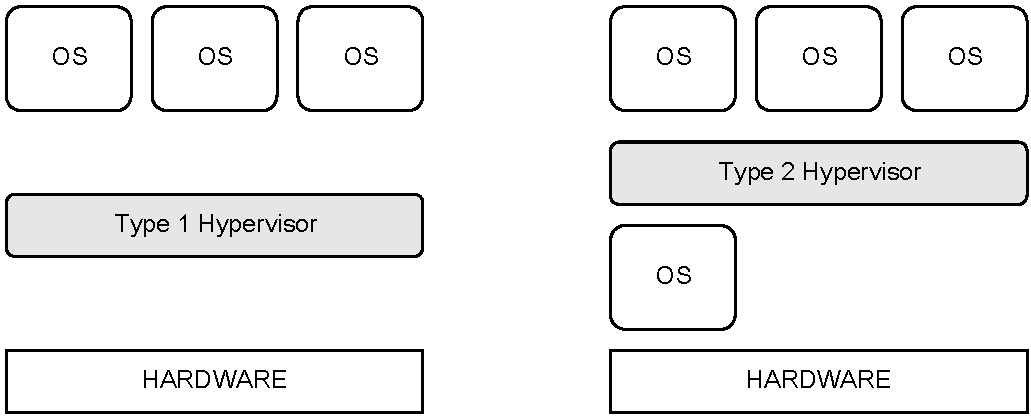
\includegraphics[scale=0.6]{images/type_hyper.pdf}
\caption{{Schema of Type 1 (native) hypervisor executing directly on physical hardware and Type 2 (hosted) hypervisor running on top of a commodity operating system}}
\label{type_hyper}
\end{center}
\end{figure}


Despite the place where an hypervisor is executing, a separation mechanism is required to run the guest operating system in a distinct software level.

In order to guarantee separation between the kernel and regular applications, traditional processors support two execution modes: operating system code runs in root mode and applications usually run in non-root mode. In the same way, the guest and the hypervisor need to be completely isolated from each other. This isolation is guaranteed by the virtualisation-enabled processor architecture.
To allow the execution of the hypervisor at a higher privilege level and of the guest without modifying its code with \emph{hypervisor awareness}, virtualisation-enabled processors have been extended with a new mode, called \emph{VMX mode}. %%%SAJJAD: Also, don't you mean "privileged" level?
In this newer architecture, the hypervisor will execute in VMX-root mode and the guest kernel will run in VMX non-root mode. 

The processor executing in VMX non-root has a restricted behaviour. Consequently, if the guest kernel executes specific instructions, a trap will be generated and control will be returned to the hypervisor. The transition from VMX non-root (guest) to VMX root (hypervisor) is usually referred to as \emph{VM exit}. The transition in the other direction, from VMX root to VMX non-root, is called \emph{VM entry}. 


\begin{figure}[htbp] 
\begin{center}
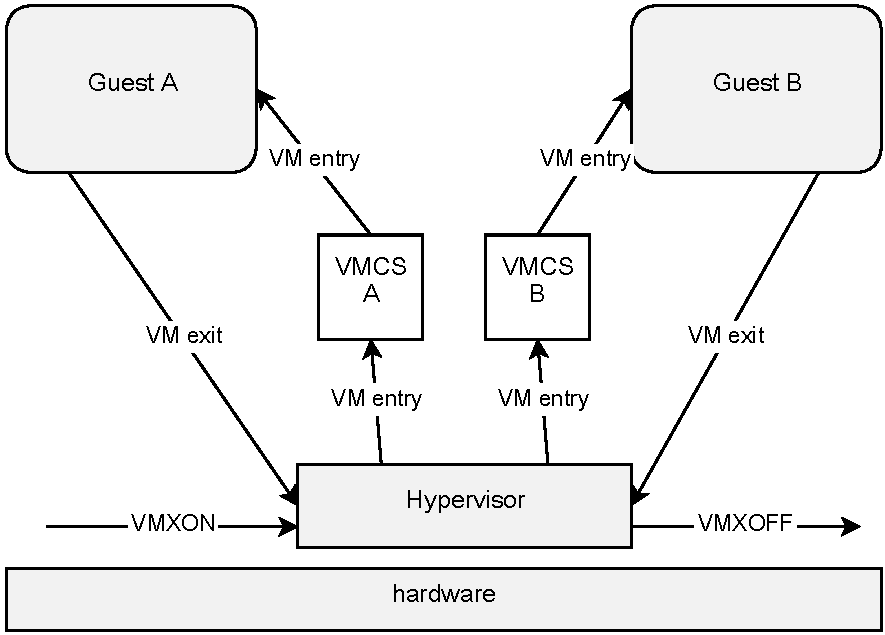
\includegraphics[scale=0.6]{images/virt_lifecycle.pdf}
\caption{{Lifecycle of a general virtual environment with two guests. When the guest executes a privileged instruction, control returns to the hypervisor by VM exit. The hypervisor executes the instruction on behalf of the guest, updates its VMCS and returns to guest's space using VM entry.}}
\label{virt_lifecycle}
\end{center}
\end{figure}

%%%SaAJJAD: Shouldn't you put a "the" before "guest's space" in the above paragraph? 

Both Intel and AMD architectures do not provide any hardware setting that is visible from the guest and that might reveal the current processor's mode. This is an effective solution to prevent guest code from detecting whether it is running on physical or virtual hardware. However, measuring the delay of specific operations with external timers\footnote{Within a virtual machine, time is shared with the hypervisor and a number of virtual machines. Each virtual machine can be preempted at any time, even when interrupt sources are disabled. This is possible because in reality only virtual interrupts are disabled. This preemption can cause a desynchronisation between virtual time and real time.} has been found to be a viable way to detect the execution of code in virtualised environments rather than on real hardware \cite{timevirt,antivirt}. 

%%%SAJJAD: in "another number of virtual" why not just say "a number of virtual" ... ALSO: Don't you mean "interruption" instead of "interrupts"?
 
%As a recurrent mechanism exploited by the countermeasures described in further chapters, we briefly explain the lifecycle of a virtualised operating system running on top of a general purpose hypervisor.
As a recurrent mechanism exploited by the countermeasures described in the proceeding chapters, we will briefly explain the lifecycle of a virtualised operating system running on top of a general purpose hypervisor. %%%SAJJAD: 

%Upon execution of the VMXON instruction, which enables the hardware-assisted virtualisation instruction set, the hypervisor enters the guest using a VM entry. At this point guest code executes until the next VM exit, by which control is transferred to a specific entry point in hypervisor space. 
Upon execution of the VMXON instruction, which enables the hardware-assisted virtualisation instruction set, the hypervisor enters the guest using a VM entry. At this point guest code executes until the next VM exit, and thus transfers control to a specific entry point in hypervisor space. %%%SAJJAD
An appropriate action is taken depending on the reason that caused the VM exit. The hypervisor usually performs the requested operation on behalf of the guest. After the execution of the privileged instruction, the hypervisor updates the context of the guest and returns using VM entry. The aforementioned mechanism is illustrated in Figure \ref{virt_lifecycle}. 

Another event that requires the hypervisor's intervention occurs when executing several virtual machines at the same time. In this case the hypervisor must restore the context of the next virtual machine to execute using instructions like $VMRESUME$ and $VMLAUNCH$. The procedure resembles the save-and-restore mechanism typical of task switching in traditional operating systems.%%%SAJJAD added "the" in "that requires hypervisor's intervention" ... I would also review the last sentence "The Mechanism ... ."

In both scenarios the context of the virtual machine is saved into a special data structure called Virtual Machine Control Structure (VMCS). The aforementioned data structure is defined \emph{special} in the sense that it is not saved into memory that is normally accessible from the guest. Moreover, special hardware instructions are needed for reading and writing to this memory area.

In general the VMCS data are organised as follows\footnote{This layout is specific to the Intel-VT architecture}:

\begin{itemize}
\item \textbf{Guest-state area} is the location in which the guest processor's state (i.e. control registers, debug registers, segment selectors, instruction pointer, but also activity and interruptibility state) is saved before returning control to the hypervisor and restored upon VM entry.

\item{\textbf{Host-state area}} is the location where the processor state of the host is loaded from, upon VM exit

\item {\textbf{VM-execution control fields}} determine the causes of VM exits and limit processor behaviour when the guest is executing, in VMX non-root mode

\item{\textbf{VM-entry control fields}} govern the behaviour of VM entries by specifying the list of MSR to be loaded or determine event injection by specifying the type of interrupt, length of instruction etc.%%%SAJJAD: "interruption" instead of "interrupt". 

\item{\textbf{VM-exit information fields}} provide basic information about VM exits such as the exit reason to be handled accordingly by the hypervisor
\end{itemize}


%The hypervisor is the only component that can shut down the virtualisation machinery and leave \emph{VMX mode} by calling the $VMXOFF$ instruction. After such an event, the processor will perform with the standard instruction set.
The hypervisor is the only component that can shut down the virtualisation machinery and leave \emph{VMX mode} by calling the $VMXOFF$ instruction. After such an event, the processor will operate with the standard instruction set.%%%SAJJAD: "operate" instead of "perform"


\begin{table}[t]
\centering
\begin{tabular}{|l|l|l|}
\hline
\bf{Instruction} & \bf{Opcode}  & \bf{Description}  \\
\hline

VMXON    & 0xF30FC7 & Enter VMX Operation \\
VMXOFF   & 0x0F01C4 & Leave VMX Operation \\
VMCALL   & 0x0F01C1 & Call to VM Monitor \\
VMLAUNCH & 0x0F01C2 & Launch Virtual Machine \\
VMRESUME & 0x0F01C3 & Resume Virtual Machine \\
VMPTRLD  & 0x0FC7   & Load Pointer to Virtual-Machine Control Structure \\
VMPTRST  & 0x0FC7   & Store Pointer to Virtual-Machine Control Structure \\
VMREAD   & 0x0F78   & Read Field from Virtual-Machine Control Structure \\
VMWRITE  & 0x0F79   & Write Field to Virtual-Machine Control Structure \\
VMCLEAR  & 0x660FC7 & Clear Virtual-Machine Control Structure \\
\hline
\end{tabular}
\caption{Intel VT-x hardware-supported virtualisation instruction set}
\label{virt:intelvt}
\end{table}

%As mentioned before, when the guest operating system is executing and the processor is in \emph{VMX non-root} mode, several events can cause control to be returned to the hypervisor. These events are treated like faults. As for any type of faults the instruction that caused it is not executed, the processor state is not updated and an action is taken by a fault handler, depending on a flag that determines the fault reason.
As mentioned before, when the guest operating system is executing and the processor is in \emph{VMX non-root} mode, several events can lead to control being returned to the hypervisor. These events are treated like faults. As for any type of fault, the instruction that caused it is not executed, the processor state is not updated and an action is taken by a fault handler, depending on a flag that determines the fault reason. %%%SAJJAD

It should be clear that in a virtualisation setting, the fault handler is represented by code running in hypervisor space. Therefore the hypervisor is responsible for the execution of additional code on behalf of the guest and for updating the guest's processor state.

\begin{figure*}[htbp] 
\begin{center}
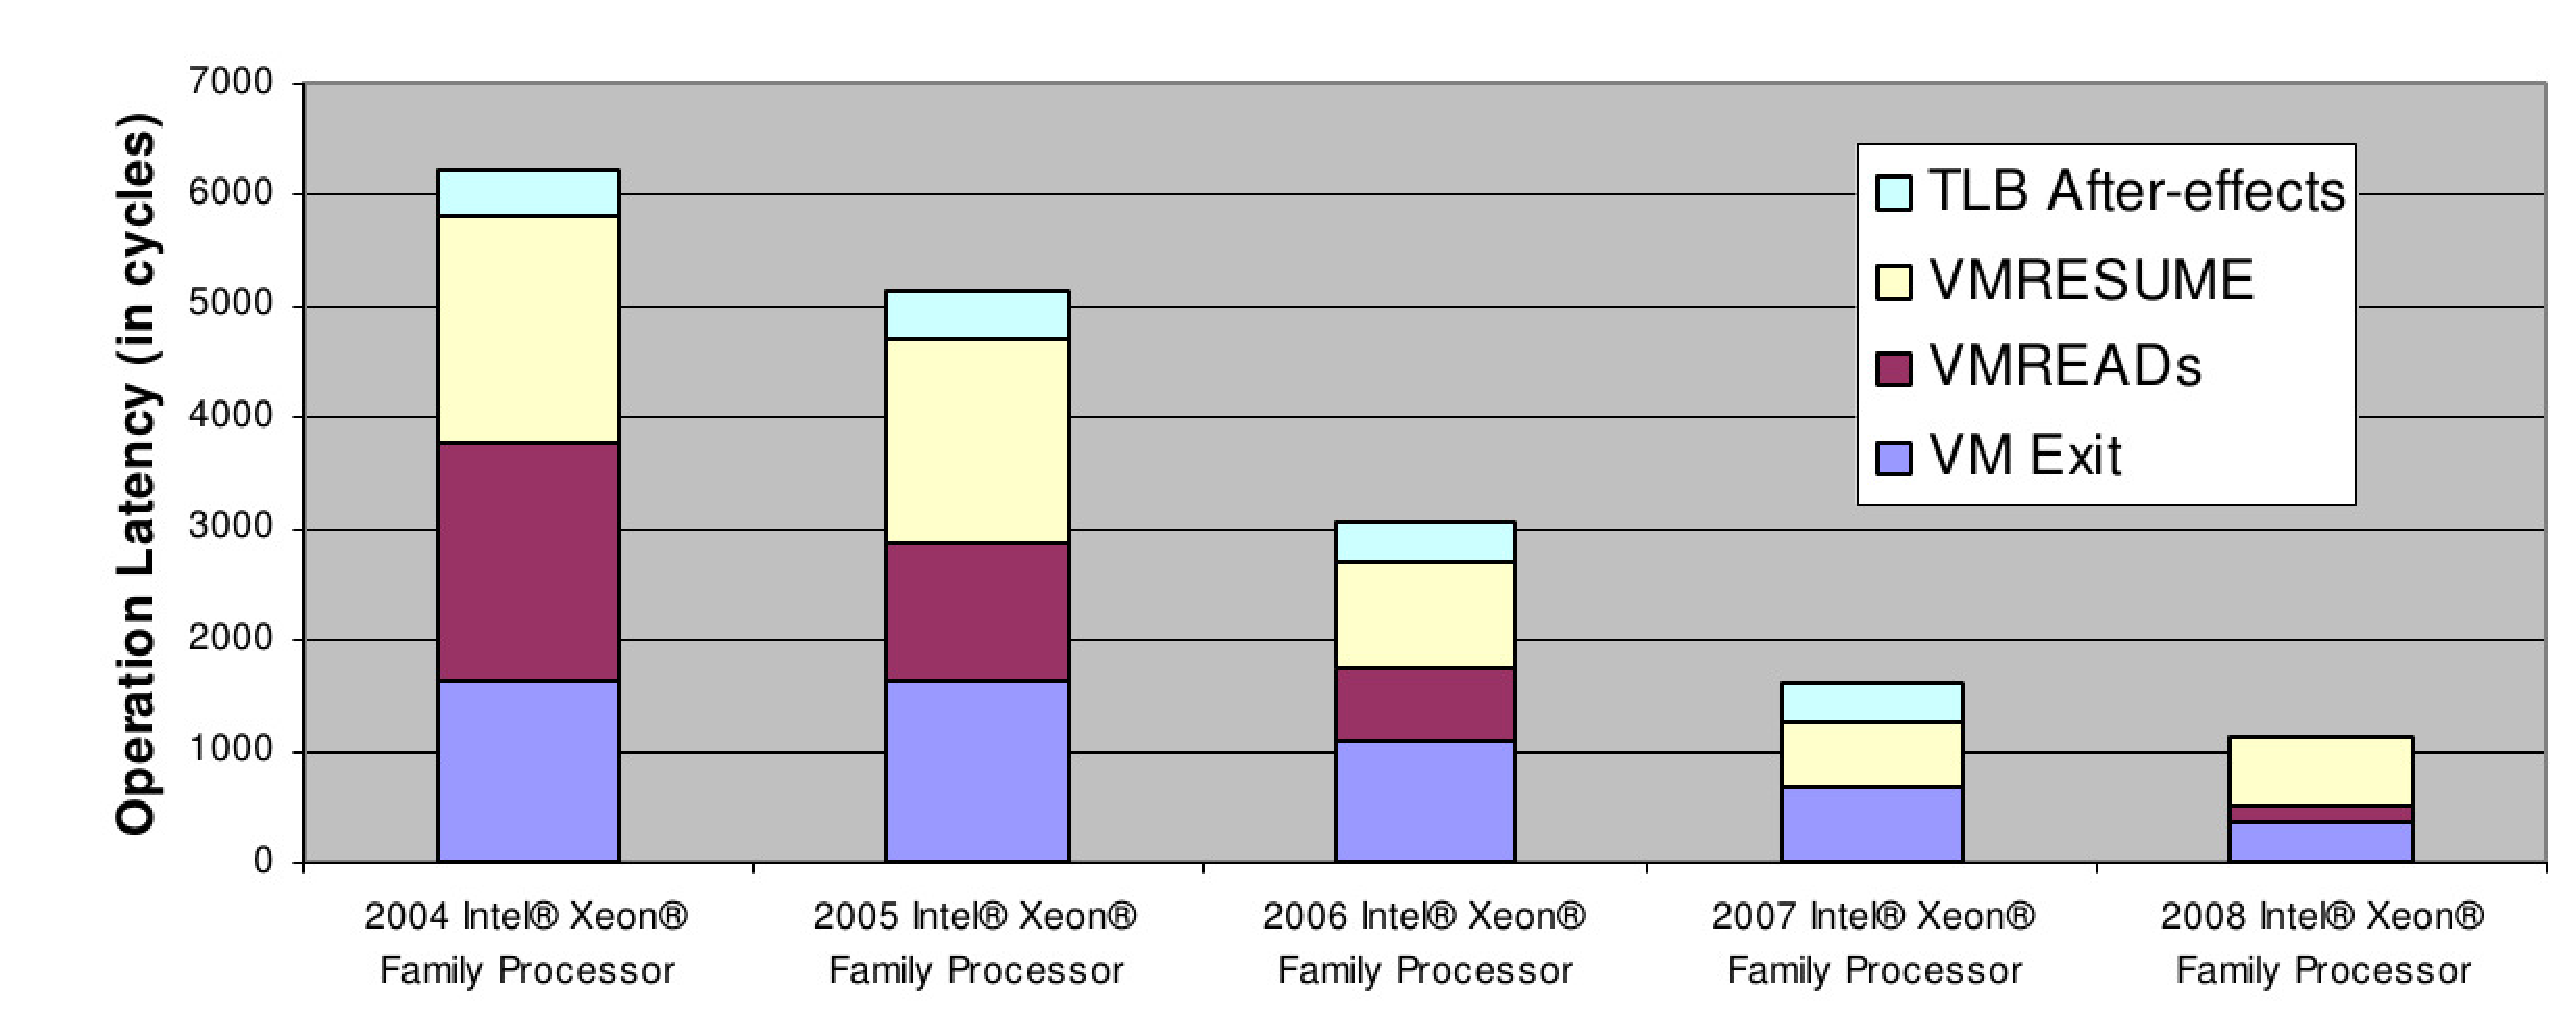
\includegraphics[scale=0.27]{images/intel_latency}
\caption{{Latency of VM exit, VMREAD, VMRESUME instructions across Intel processors}}
\label{intel_latency}
\end{center}
\end{figure*}


A list of instructions that cause VM exit when the processor is in \emph{VMX non-root} mode is reported in Table \ref{virt:insntrap}. Other events that are handled with the same trapping mechanism are exceptions, external interrupts (otherwise served by the guest Interrupt Descriptor Table), non-maskable (NMI) and system-management (SMI) interrupts and task switches. For a more detailed description about how to handle VM exits and other architecture specific features of virtualisation-enabled processors we encourage the reader to examine the architecture developer's manual, usually provided by the hardware vendor.

\begin{table}[t]
\centering
\begin{tabular}{|l|l|l|}
\hline
\bf{Instruction} & \bf{Opcode}  & \bf{Description}  \\
\hline
\texttt{Unconditionally VMExit}  \\
\hline
CPUID          & 0xF30FC7 & Enter VMX Operation \\
INVD           & 0x0F01C4 & Leave VMX Operation \\
MOV from CR3   & 0x0F01C1 & Call to VM Monitor \\
VM* insn & & All instructions in the \\
& & VM extended instruction set \\
\hline
\texttt{Conditionally VMExit}  \\
\hline
CLTS          & 0x0F01C2 & Clear Task-Switched Flag in CR0 \\
HLT           & 0x0F01C3 & Halt \\
IN,INS*       &          & Input from Port to String \\
OUT,OUTS*     &          & Output String to Port \\
INVLPG        & 0x0F017  & Invalidate TLB Entry \\
LMSW          & 0x0F016  & Load Machine Status Word \\
MONITOR       & 0x0F01C8 & Set Up Monitor Address \\
MOV from CR8  &          & Move from Control Register 8 \\
MOV to CR0/CR3/CR4/CR8  && Move to Control Register 0,3,4,8 \\
MOV DR  & 0x660FC7   & Move to Debug Register \\
MWAIT   & 0x0F01C9   & Monitor Wait  \\
PAUSE   & 0xF390     & Spin Loop Hint \\
RDMSR   & 0x0F32     & Read from Model Specific Register \\
RDPMC   & 0x0F33     & Read Performance-Monitoring Counters \\
RDTSC   & 0x0F31     & Read Time-Stamp Counter \\
RSM     & 0x0FAA     & Resume from System Management Mode \\
WRMSR   & 0x0F30     & Write to Model Specific Register \\
\hline
\end{tabular}
\caption{List of privileged instructions that cause a VMExit event}
\label{virt:insntrap}
\end{table}

\clearpage
\subsection{Performance}
The high complexity of the trapping mechanism has an impact on the overall performance of the system. Even for hardware-assisted virtualisation, VM exits are expensive. 
   
%Introduce the costs of trapping in terms of clock cycle and latency \\ 
%...Hence, the cost of VMentry and VMexit is an important factor in the performance of implementation methods for system virtualisation.
\emph{Para-virtualisation} has been introduced as a way to reduce the latencies of the trapping mechanism. Para-virtualisation is a technique in which the hypervisor provides an API to the guest operating system. A guest using the API, instead of the regular trapping mechanism, will result in an increase in the overall performance due to the reduced number of traps. In fact, some mechanisms that usually need the interposition of the hypervisor could be executed directly from the guest. In work such as \cite{virtio, HPC, xenart} it is shown how to para-virtualise device drivers in order to considerably improve I/O-intensive tasks.%%%SAJJAD "will result to increased" replaced with "will result in an increase in the"
 
Para-virtualisation, however, usually requires guest kernel code to be modified. This last requirement cannot always be fulfilled, especially when source code is not available, as is the case of proprietary operating systems. On the other hand, hardware-supported virtualisation can rely on entirely unmodified guest operating systems, something that usually involves many more VM traps and thus higher CPU overheads.%%%SAJJAD

One of the main issues of memory virtualisation is that in order to guarantee isolation, guests cannot access physical memory directly. Therefore, in addition to virtualising the processor unit, memory virtualisation is also required. This is a critical component that influences the performance impact of memory-intensive virtualised applications. 

In a standalone operating system, the hardware Memory Management Unit (MMU) is used to map logical page addresses (LPA) to the physical page addresses (PPA). To achieve faster lookups, the Translation Lookaside Buffer (TLB) caches the most recently used $LPA \rightarrow PPA$ mappings, for future access.%%%SAJJAD: "access" instead of "accesses"


\begin{figure}[htbp] 
\begin{center}
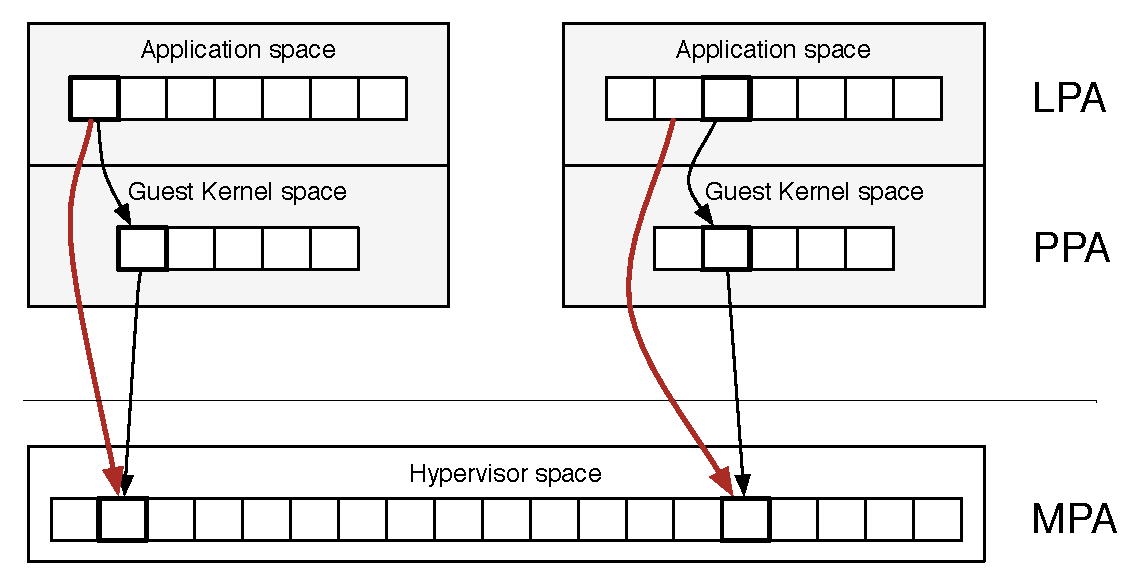
\includegraphics[scale=0.6]{images/shadow.pdf}
\caption{{Schema of two-level translation from LPA (Logical Page Address) to PPA (Physical Page Address) and MPA (Machine Page Address).  Red arrows indicate the mappings from guest to host that the hypervisor must keep synchronised in its shadow pages.}}
\label{shadow}
\end{center}
\end{figure}



This mechanism holds in a virtualised environment, but an additional layer is necessary in order to map a PPA to a machine page address (MPA). The two-level translation mechanism is illustrated in Figure \ref{shadow}.%%%SAJJAD: By "hold" you mean "takes place"?


Prior to the advent of hardware-supported virtualisation, the hypervisor had to maintain $PPA \rightarrow MPA$ mappings and had to store $LPA \rightarrow MPA$ mappings in \emph{shadow page tables}. Faster lookups could be achieved by caching $LPA \rightarrow MPA$ mappings into the TLB. Unfortunately, whenever the guest re-mapped its memory addresses, the hypervisor had to keep the shadow pages synchronised. This task was recognised as the factor responsible for most of the performance impact of the technology.%%%SAJJAD: I added "the factor"



\begin{figure}[htbp] 
\begin{center}
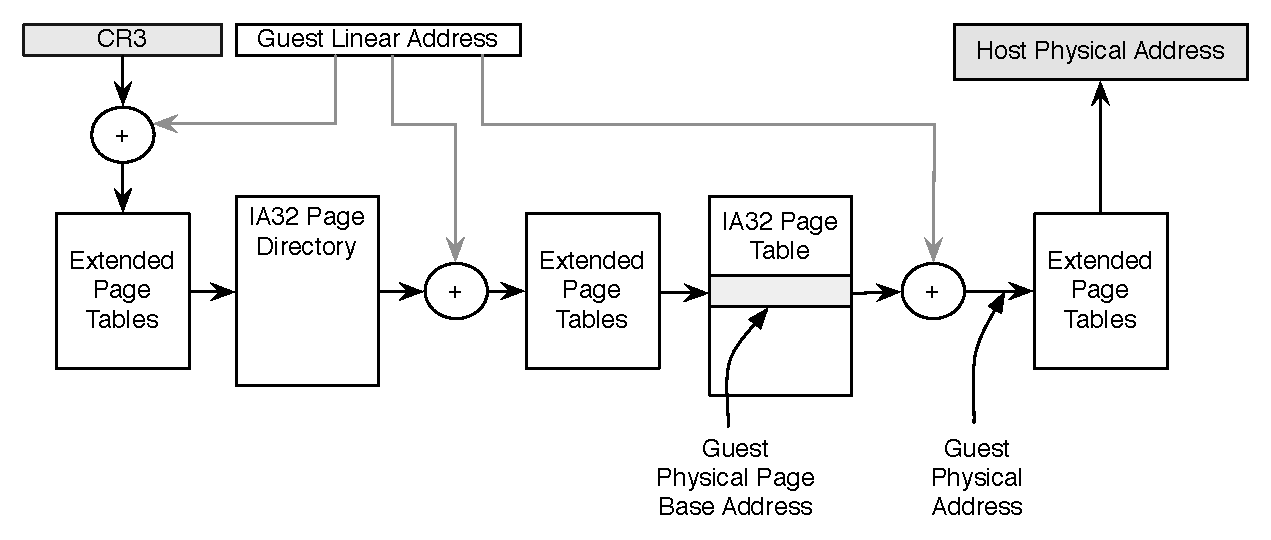
\includegraphics[scale=0.6]{images/EPT.pdf}
\caption{{Intel's Extended Page Table hardware-supported translation mechanism to map guest addresses to host physical addresses without shadow paging. An equivalent method has been developed by AMD, with the name of NPT (Nested Page Tables)}}
\label{EPT}
\end{center}
\end{figure}


Lately, vendors like AMD and Intel included hardware support for memory virtualisation, called AMD Nested Page Tables (NPT) and Intel Extended Page Tables (EPT)  respectively.\\ %%%SAJJAD: relocated "respectively"
In this second scenario (Figure \ref{EPT}), any access to a logical page from within the guest triggers the composite translation of both $LPA \rightarrow PPA$ and $PPA \rightarrow MPA$. Therefore no shadow pages are needed and data will be kept synchronised without additional overhead. Clearly, the cost of a page walk needed for the double translation is slightly higher with respect to the one performed with traditional page tables\footnote{The use of large pages when NPT/EPT is enabled reduces the overall impact inflicted by the higher cost of page walks, as it has been measured in \cite{perfEPT, perfESX} }.  


The non-negligible performance impact introduced by the technology should always be taken into consideration for correctly designing infrastructures that rely heavily on virtualisation.%%%SAJJAD: "rely heavily" instead of "heavily rely"  (both are kinda correct, but this is better)

A mechanism that allows the guest operating system to return control to the hypervisor synchronously is referred to as \emph{hypercall}. A hypercall is the equivalent of a system call in traditional operating systems. 
For instance, in order to invoke a system call on UNIX systems, the program in user space pushes the value of the system call in register EAX and then raises an interrupt. A sequence of instructions that explain the mechanism is shown in Listing \ref{syscall}

\begin{lstlisting} [caption=A simple system call in traditional UNIX, label= syscall]
mov eax, 1
push eax
int 80h
\end{lstlisting}

When interrupt \emph{80h} is raised the kernel interrupt handler will read the value of register EAX, which in turn jumps to the handler of the system call (in the example above it will be system call 1) and executes it with the parameters popped from the stack.
The mechanism of hypercalls is very similar to the one of a system call. The main difference is that an interrupt different from \emph{80h} is raised. The interrupt number depends on the hypervisor's design.
Hypercalls are commonly used in \emph{para-virtualised} systems in which execution jumps directly from the application (Ring 3) to the hypervisor, which then passes control to the guest kernel (Ring 0). 

However, hypercalls are also used in systems that are not hypervisor aware, whenever it is required to return control to the hypervisor explicitely. In fact, hypercalls are handled by the hypervisor synchronously, which means that execution of the guest operating system will be paused until the handler terminates.
Despite the performance penalty of the hypercall mechanism, it revealed to be extremely useful in several cases  presented throughout this work.

%This performance hit can be mitigated by the use of paravirtualized drivers; the combination has been called "hybrid virtualisation".[4]
%Hypercall mechanism used throughout this work represents a hybrid virtualisation mechanism: kernel extension and hypervisor API (or protocol) \\ 


\section{Benefits and drawbacks}
%The numerous advantages introduced by virtualisation technology are influencing several aspects of designing modern computing infrastructure. Hardware engineers are improving virtualisation-supported processors at a constant pace, reducing what was used to be a considerable gap between performance of software running on real hardware and in virtualisation environments.
The numerous advantages introduced by virtualisation are influencing several aspects of designing modern computing infrastructure. Hardware engineers are improving virtualisation-supported processors at a constant pace, reducing what used to be a considerable gap between the performance of software running on real hardware and those in virtualisation environments.%%%SAJJAD

Despite ample room for the improvement of the latency of complex instructions, like the ones offered by the virtualisation instruction set, server consolidation, one of the most frequent applications of virtualisation technology in the industry, is contributing to a much more efficient usage of computing resources. The significant reduction of energy consumption is a benefit that comes as a direct consequence. Server consolidation addresses the reduction of existing infrastructure \cite{consolidation}. Moreover, less physical hardware also leads to lower management costs (such as the costs of regular wearing, faulty hardware, etc.) 
%It goes without saying that it is the reduction of these types of costs that triggered the migration to virtualised data centres in the early days and encouraged other users to do so, later on
It goes without saying that it is the reduction of these types of costs that triggered the migration to virtualised data centres in the early days and encouraged other users to follow later on.%%%SAJJAD

The natural course of hardware development and the popularity of virtualisation technology promoted the replacement of traditional processors with new hardware. Today, virtualisation-supported processors are off-the-shelf components regularly installed on general purpose computers. Therefore, virtualisation-friendly solutions meet their requirements with much more ease than in the past when they could be deployed only when accompanied with special hardware.


Despite the benefits described above, which might be interpreted more as business-related advantages, a feature that is rendering virtualisation technology even more attractive from a more technical view point, is the inherent isolation of virtual machines from themselves and the hypervisor. The need for executing several guests at the same time and preventing any type of interference are requirements that cannot be fulfilled without isolation.

As explained in Section \ref{virt:tech}, it should be clear that hardware-support is not only beneficial to the overall performance impact\footnote{The benefit becomes consistent when hardware-supported virtualisation is compared to software emulation. But compared to a native system, a virtualisation solution continues to have non-negligible impact.} but also to security. In a hardware-assisted virtualisation framework it is substantially hard - sometimes not practically feasible - to break the isolation constraint from within a virtual machine. 
%This particular feature, which comes by design, is broadening those researchers' horizons who provide security solutions based on sandboxes or similar isolation environments.
This particular feature, which comes by design, is broadening the horizon of those researchers who provide security solutions based on sandboxes or similar isolation environments.%%% SAJJAD
 

Apart from the use of virtualisation as a way to host different operating systems on a single physical machine, virtualisation is currently also being used to provide greater security guarantees for operating system kernels.
This specific scenario will be described extensively in Chapter \ref{hellorootkitty} and Chapter \ref{hyperforce}.

%Condensing several physical machines into fewer well-dimensioned ones (energy efficiency) \\ 
%Management costs (less hardware required for server consolidation, better maintenance, creating, destroying, migrating machines) \\
%Hardware-supported virtualisation guarantees complete isolation among virtual machines reducing performance overhead with respect to virtualisation-by-emulation \\
%[drawbacks]\\
However, moving the direct control of physical hardware to the lower level of the hypervisor, and delegating to this only component all critical operations with the purpose of arbitrating the execution of the guests, might lead to security issues. Obviously, a bug within hypervisor code might affect the entire virtualisation platform. 
A general strategy to avert such an issue involves keeping the hypervisor's code size as small as possible in order to increase the chances to discover bugs and provide fixes at the earliest.
 
Formal verification techniques can be considered, in order to prevent possible faults or unexpected behaviour from hypervisor space. However, these solutions are feasible only under simple assumptions, most of the times when hypervisor code has been written with verification in mind. 
The challenging part of the verification task becomes more evident since hypervisors are usually written in unsafe languages (such as C and assembly code for performance reasons) with an easily circumvented type system and explicit memory allocation. For such systems, memory safety has to be verified explicitly. Moreover, the hypervisor is usually formed by code that runs concurrently and address translations occur asynchrounously and non-atomically \cite{formalmethods,verifyhyperv}.  
Last but not least, virtualisation strategies that can fully exploit the hardware to execute a multitude of guest operating systems with high performance, require the hypervisor to execute directly on physical hardware. This can increase the size of the hypervisor (a large code base is usually represented by device drivers) and make verification a non-tractable task. However, there have been attempts to formally verify hypervisors with a small codebase, a task that is more accessible than verifying commodity operating systems \cite{hyperv, formsecxenon}.   
%%%SAJJAD "consists in" replaced with "involves"

%Bottleneck of the entire system in terms of performance and security is shifted to a higher privilege level (hypervisor) (if buggy hypervisor, the entire system (not only the hypervisor but also all virtual machines running on top) is at risk) \\

Despite the performance improvements claimed by works like \cite{rearch, avoidvmexit} and by Intel itself, as shown in Figure \ref{intel_latency}, the gap of the performance between native and virtualised operating systems remains consistent.  
It is clear that the performance impact is mainly caused by the latency of virtualisation-based instructions, which is mainly architecture dependent. The frequency of trapped events from the guest to the hypervisor is also important and it has been measured to have a considerable impact on the overall performance of a virtualised system, specially affecting Input/Output intensive tasks. In \cite{avoidvmexit}, this frequency has been minimised using software techniques. In the same work it is claimed that the overall transition costs are reduced up to 50\%. However, the aforementioned latency seems to be improvable up to a lower bound imposed by the technology. %%%SAJJAD: check first sentence

%http://www.anandtech.com/show/2480/9
%Although overhead has been reduced consistently by hardware support, performance impact is still not negligible, specially for I/O intensive tasks (virtualized operating systems run on additional software level rather than bare metal) \\

\section{Rethinking security} \label{rethinking}
One of the immediate effects of the advent of virtualisation into marketplace is the new way of thinking about security. The desire to exploit this new environment and deal with challenging and unsolved problems - mainly related to operating system kernel security - is so intense that several security solutions promptly appeared in the literature \cite{9, hvmharvard, NICKLE, dynamicdatakernel}.      
However, protecting operating system kernels from being compromised is challenging and still an open problem. 
Virtualisation offers viable ways to mitigate these types of threats. However, due to the significant overhead introduced by the technology, any security solution needs to be designed with performance in mind.

We provide a realistic model of attack to operating system kernels and a strategy to detect attacks of this type when the operating system has been virtualised, in Chapter \ref{hellorootkitty}. 

Still in the field of kernel security, a more general framework that enforces the execution of monitoring code within a virtualised operating system is described in Chapter \ref{hyperforce}. 
It will be shown that the performance impact of our solutions is negligible and limited by the lower bound of the technology.

The role of virtualisation technology to improve the security of web browsers and applications delivered on-demand is described in Chapter \ref{bubble}.
